% !TeX spellcheck = en_US
%\documentclass[11pt,a4paper]{article}
\documentclass[11pt
  , a4paper
  , article
  , oneside
%  , twoside
%  , draft
]{memoir}

\usepackage{control}
\usepackage{kotex}
\usepackage[numbers]{natbib}
%\usepackage[pdftex]{graphicx}
%\DeclareGraphicsExtensions{.pdf,.png,.jpg}
\begin{document}

\newcommand{\technumber}{
  Digital Signal Processing using MATLAB\\
  Document 1: 2016-03-26}
\title{\textbf{Digital Signal Processing: 실습 4 \\
		제3장 이산시간 푸리에  변환의 성질 \\}}

\author{이상일\thanks{silee7103@ibs.re.kr} \\

  학번: 201460437\\
  Computer Engineering, Chungnam National University 
}
\date{\today}

\renewcommand{\maketitlehooka}{\begin{flushright}\textsf{\technumber}\end{flushright}}
%\renewcommand{\maketitlehookb}{\centering\textsf{\subtitle}}
%\renewcommand{\maketitlehookc}{C}
%\renewcommand{\maketitlehookd}{D}

\maketitle

\begin{abstract}
MATLAB을 사용한 Digital Signal Processing에 대한 실습과제에 대한 Documents를 구성한다.
\end{abstract}

\chapter{Example 3-3:}

\begin{lstlisting}[style=termstyle]
% Example 3.3
w = [0:1:500]*pi/500;  
X = exp(j*w) ./ (exp(j*w) - 0.5*ones(1,501));
magX = abs(X); angX = angle(X); realX = real(X); imagX = imag(X);

subplot(2,2,1); plot(w/pi,magX); grid
xlabel('frequency in pi units'); title('Magnitude Part'); ylabel('Magnitude')
subplot(2,2,3); plot(w/pi,angX); grid
xlabel('frequency in pi units'); title('Angle Part'); ylabel('Radians')
subplot(2,2,2); plot(w/pi,realX); grid
xlabel('frequency in pi units'); title('Real Part'); ylabel('Real')
subplot(2,2,4); plot(w/pi,imagX); grid
xlabel('frequency in pi units'); title('Imaginary Part'); ylabel('Imaginary')
\end{lstlisting}

\begin{figure}[h!]
	\centering
	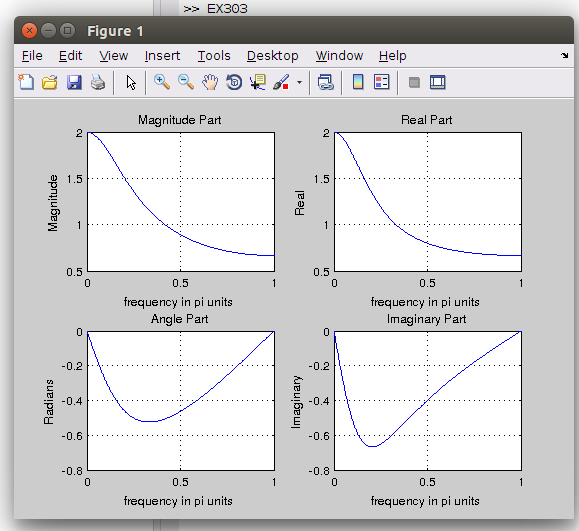
\includegraphics[width=0.7\textwidth,height=0.2\textwidth]{./images/Ex3-3.png}
	\caption{Example 3.3 Result}
	\label{fig:Example 3-3 Result}
\end{figure}


\chapter{Example 3-4:}

\begin{lstlisting}[style=termstyle]
% Example 3.4:
n = -1:3; x = 1:5; 
k = 0:500; w = (pi/500)*k; 
X = x * (exp(-j*pi/500)) .^ (n'*k); 

magX = abs(X); angX = angle(X);
realX = real(X); imagX = imag(X);

subplot(2,2,1); plot(w/pi,magX); grid
xlabel('frequency in pi units'); title('Magnitude Part'); ylabel('Magnitude')
subplot(2,2,3); plot(w/pi,angX); grid
xlabel('frequency in pi units'); title('Angle Part'); ylabel('Radians')
subplot(2,2,2); plot(w/pi,realX); grid
xlabel('frequency in pi units'); title('Real Part'); ylabel('Real')
subplot(2,2,4); plot(w/pi,imagX); grid
xlabel('frequency in pi units'); title('Imaginary Part'); ylabel('Imaginary')
\end{lstlisting}

\begin{figure}[h!]
	\centering
	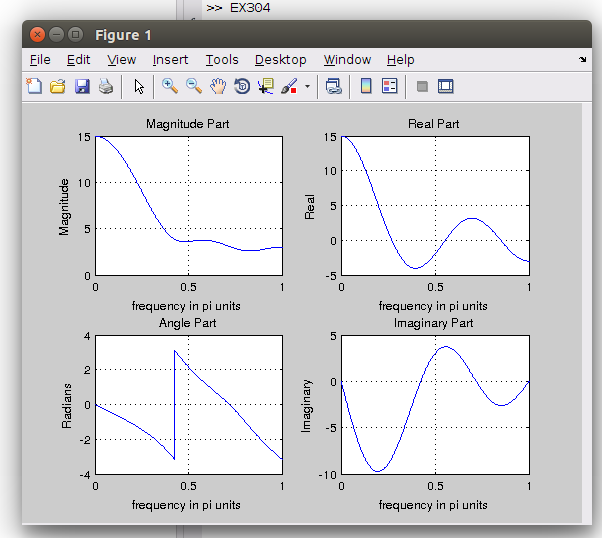
\includegraphics[width=0.7\textwidth,height=0.5\textwidth]{./images/Ex3-4.png}
	\caption{Example 3.4 Result}
	\label{fig:Example 3-4 Result}
\end{figure}

\clearpage

\chapter{Example 3-5:}
\begin{lstlisting}[style=termstyle]
%Example 3.5
n = 0:10; x = (0.9*exp(j*pi/3)).^n;
k = -200:200; w = (pi/100)*k;
X = x * (exp(-j*pi/100)) .^ (n'*k);

magX = abs(X); angX =angle(X);

subplot(2,1,1); plot(w/pi,magX);grid
axis([-2,2,0,8])
xlabel('frequency in units of pi'); ylabel('|X|')
title('Magnitude Part')

subplot(2,1,2); plot(w/pi,angX/pi);grid
axis([-2,2,-1,1])
xlabel('frequency in units of pi'); ylabel('radians/pi')
title('Angle Part')
\end{lstlisting}

\begin{figure}[h!]
	\centering
	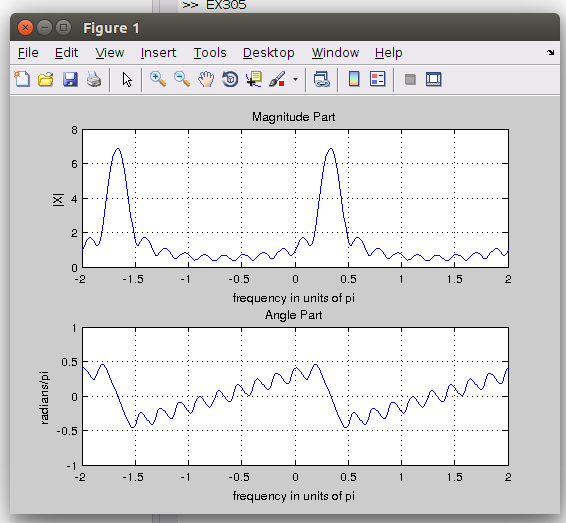
\includegraphics[width=0.7\textwidth,height=0.35\textwidth]{./images/Ex3-5.png}
	\caption{Example 3.5 Result}
	\label{fig:Example 3-5 Result}
\end{figure}

\clearpage

\chapter{Example 3-6:}
\begin{lstlisting}[style=termstyle]
%Example 3.6
n = -5:5; x = (-0.9).^n;
k = -200:200; w = (pi/100)*k;
X = x * (exp(-j*pi/100)) .^ (n'*k);

magX = abs(X); angX =angle(X);

subplot(2,1,1); plot(w/pi,magX);grid
axis([-2,2,0,15])
xlabel('frequency in units of pi'); ylabel('|X|')
title('Magnitude Part')

subplot(2,1,2); plot(w/pi,angX/pi);grid
axis([-2,2,-1,1])
xlabel('frequency in units of pi'); ylabel('radians/pi')
title('Angle Part')
\end{lstlisting}

\begin{figure}[h!]
	\centering
	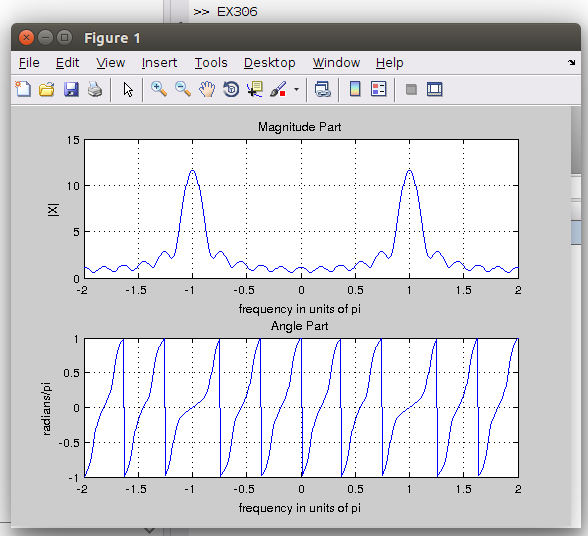
\includegraphics{./images/Ex3-6.png}
	\caption{Example 3.6 Result}
	\label{fig:Example 3-6 Result}
\end{figure}

\clearpage

\chapter{Example 3-7:}
\begin{lstlisting}[style=termstyle]
%Example 3.7

x1 = rand(1,11); x2 = rand(1,11); n = 0:10;
alpha = 2; beta = 3;
k = 0:500; w = (pi/500)*k;
X1 = x1 * (exp(-j*pi/500)).^(n'*k); 
X2 = x2 * (exp(-j*pi/500)).^(n'*k); 

x = alpha*x1 + beta*x2;             
X = x * (exp(-j*pi/500)).^(n'*k);   

X_check = alpha*X1 + beta*X2;       
error = max(abs(X-X_check))         
\end{lstlisting}

\begin{figure}[h!]
	\centering
	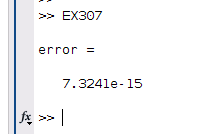
\includegraphics[width=0.4\textwidth,height=0.15\textwidth]{./images/Ex3-7.png}
	\caption{Example 3.7 Result}
	\label{fig:Example 3-7 Result}
\end{figure}

\chapter{Example 3-8:}
\begin{lstlisting}[style=termstyle]
%Example 3.8

x = rand(1,11); n = 0:10;
k = 0:500; w = (pi/500)*k;
X = x * (exp(-j*pi/500)).^(n'*k); 

y = x; m = n+2;
Y = y * (exp(-j*pi/500)).^(m'*k); 

Y_check = (exp(-j*2).^w).*X;      
error = max(abs(Y-Y_check))    
\end{lstlisting}

\begin{figure}[h!]
	\centering
	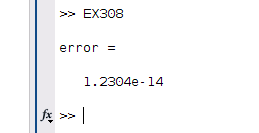
\includegraphics[width=0.4\textwidth,height=0.15\textwidth]{./images/Ex3-8.png}
	\caption{Example 3.8 Result}
	\label{fig:Example 3-8 Result}
\end{figure}


\chapter{Example 3-9:}
\begin{lstlisting}[style=termstyle]
%Example 3.9

n = 0:100; x = cos(pi*n/2);
k = -100:100; w = (pi/100)*k;        % frequency between -pi and +pi
X = x * (exp(-j*pi/100)).^(n'*k);    % DTFT of x

y = exp(j*pi*n/4).*x;                % signal multiplied by exp(j*pi*n/4)
Y = y * (exp(-j*pi/100)).^(n'*k);    % DTFT of y

subplot(1,1,1)
subplot(2,2,1); plot(w/pi,abs(X)); grid; axis([-1,1,0,60])
xlabel('frequency in pi units'); ylabel('|X|')
title('Magnitude of X')

subplot(2,2,2); plot(w/pi,angle(X)/pi); grid; axis([-1,1,-1,1])
xlabel('frequency in pi units'); ylabel('radiands/pi')
title('Angle of X')

subplot(2,2,3); plot(w/pi,abs(Y)); grid; axis([-1,1,0,60])
xlabel('frequency in pi units'); ylabel('|Y|')
title('Magnitude of Y')

subplot(2,2,4); plot(w/pi,angle(Y)/pi); grid; axis([-1,1,-1,1])
xlabel('frequency in pi units'); ylabel('radians/pi')
title('Angle of Y')
\end{lstlisting}

\begin{figure}[h!]
	\centering
	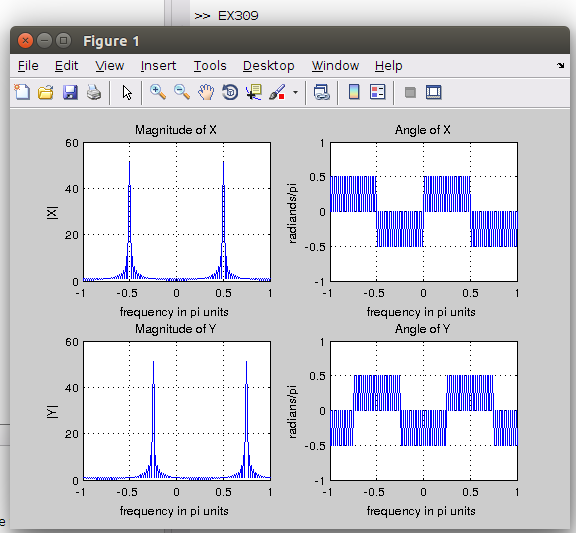
\includegraphics[width=0.7\textwidth,height=0.5\textwidth]{./images/Ex3-9.png}
	\caption{Example 3.9 Result}
	\label{fig:Example 3-9 Result}
\end{figure}

\clearpage

\chapter{Example 3-10:}
\begin{lstlisting}[style=termstyle]
%Example 3.10

n = -5:10; x = rand(1,length(n)) + j*rand(1,length(n));
k = -100:100; w = (pi/100)*k;        
X = x * (exp(-j*pi/100)).^(n'*k);    

y = conj(x);                         
Y = y * (exp(-j*pi/100)).^(n'*k);    

Y_check = conj(fliplr(X));           
error = max(abs(Y-Y_check))  
\end{lstlisting}

\begin{figure}[h!]
	\centering
	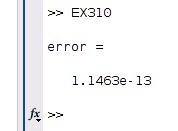
\includegraphics[width=0.4\textwidth,height=0.15\textwidth]{./images/Ex3-10.png}
	\caption{Example 3.10 Result}
	\label{fig:Example 3-10 Result}
\end{figure}

\end{document}

